\documentclass[a4paper,10pt,twocolumn]{ltjsarticle}
\usepackage[haranoaji]{luatexja-preset}
\usepackage[top=18mm,bottom=20mm,left=17mm,right=17mm,columnsep=8mm]{geometry}
\usepackage{graphicx,booktabs,array,caption,enumitem,xcolor,tikz}
\usetikzlibrary{shapes.geometric}
\setlength{\parindent}{1\zw}
\renewcommand{\baselinestretch}{1.0}
\setlength{\parskip}{0pt}
\renewcommand{\thesection}{\arabic{section}.}
\renewcommand{\thesubsection}{\arabic{section}.\arabic{subsection}.}
\makeatletter
\renewcommand{\section}{\@startsection{section}{1}{\z@}{1.1\Cvs \@plus.4\Cdp \@minus.2\Cdp}{.5\Cvs \@plus.2\Cdp}{\normalfont\gtfamily\bfseries\large}}
\renewcommand{\subsection}{\@startsection{subsection}{2}{\z@}{.8\Cvs \@plus.3\Cdp \@minus.2\Cdp}{.3\Cvs \@plus.1\Cdp}{\normalfont\gtfamily\bfseries\normalsize}}
\makeatother
\captionsetup{font={small,sf},labelsep=space,justification=raggedright,singlelinecheck=false,skip=3pt}
\captionsetup[table]{position=top}
\setlist[itemize]{leftmargin=1.2\zw,itemsep=0pt,topsep=2pt,parsep=0pt}
\setlength{\textfloatsep}{8pt plus 2pt minus 2pt}
\setlength{\floatsep}{8pt plus 2pt minus 2pt}
\setlength{\intextsep}{8pt plus 2pt minus 2pt}
\pagestyle{plain}
\raggedbottom
\begin{document}
\twocolumn[{
\noindent\fbox{\gtfamily\small\ 生成AI論文\ }\par\medskip
\begin{center}
{\gtfamily\bfseries\LARGE 好き・自信・価値を同時に見ると，得点との関連はどう変わるか：TIMSS 2023の中2を重回帰とパス解析で整理する$^{\dagger}$}\par\medskip
{\gtfamily\bfseries\large 中2の「とても好き」「とても自信あり」「とても価値あり」の割合と平均得点の，43の国・地域間の関連}\par\medskip
{\normalsize EduData調査研究グループ$^{*1}$・教育データサイエンス解析班$^{*2}$}\par
{\small オープン教育統計推進プロジェクト$^{*1}$・初等中等STEM教育データ基盤ユニット$^{*2}$}
\end{center}\smallskip
\noindent\begin{minipage}{\textwidth}\small 本研究は，TIMSS 2023の公表値から，中2の算数・数学で「とても好き」「とても自信あり」「とても価値あり」と答えた生徒の割合と平均得点の関連を，43の国・地域で整理した．1つずつ見ると，「好き」（\textit{r}=-.67）と「価値」（\textit{r}=-.74）は得点と負に関連し，「自信」の関連は確認できなかった（\textit{r}=.12）．3つを同時に入れた重回帰では，「価値」のβは-.933（95\%CI [-1.61, -.35]），「好き」のβは.172（[-.45, .81]）で，両者は強く相関し（\textit{r}=.93），分けて推定できなかった．パス解析の適合は良かったが，補数の組を含むSEMの適合は悪かった（CFI=.832，RMSEA=.399）．いずれも国・地域間の集計値の関連で，個々の生徒の因果を示さない．\par\smallskip
\noindent{\gtfamily キーワード：}TIMSS 2023，学習意欲，重回帰，パス解析，構造方程式モデリング\end{minipage}\medskip
}]
\let\thefootnote\relax
\footnotetext{\footnotesize 2026年10月執筆\\ $^{\dagger}$How Do Associations with Scores Change When Liking, Confidence and Value Are Considered Together? Multiple Regression and Path Analysis of TIMSS 2023 Grade 8†\\ $^{*1}$ Open Education Data Project, Tokyo, Japan\quad $^{*2}$ Educational Data Science Unit, Tokyo, Japan}
\section{はじめに}
\subsection{研究の背景}
算数・数学を好む程度，自信，価値の認識は，学習への関わりや達成と結びつけて論じられてきた．Bandura (1997)は自己効力感を，Wigfield and Eccles (2000)は期待と価値を，Pekrun (2006)は達成感情を，それぞれ動機づけを考える枠組みとして整理した．Lee and Stankov (2018)はTIMSSとPISAで，非認知的な特性と学業成績の関連を検討した．国を単位にすると様子が異なりうる．Shen and Tam (2008)は，TIMSSの3回の調査で，学力と自己認識の逆説的な関係を国際比較で示した．Marsh and Hau (2003)は，学力選抜のある学校が学業的自己概念に及ぼす負の効果を26か国で検討した．

TIMSS 2023の結果はIEA (2024)が報告し，2019年の結果はMullis et al. (2020)にある．回答は自己申告で，Chen et al. (1995)は，評定尺度の回答の仕方が東アジアと北米の生徒で異なることを論じた．
\subsection{リサーチクエスチョン}
本研究の目的は，中2の「好き」「自信」「価値」の割合と平均得点の，国・地域間の関連を整理することである．
\begin{itemize}
\item RQ1：3つの割合を同時に説明変数にすると，平均得点との関連は，1つずつ見たときと比べてどう変わるか（重回帰）．
\item RQ2：「好き」「価値」「得点」の関連は，パス解析と潜在変数を含むSEMでどう整理でき，適合はどうか（探索的に）．
\end{itemize}
\section{調査対象および分析方法}
IEA (2024)のExhibit 6.2.2〜6.2.8, 1.1.1, 1.2.1の公表値から，小4（58の国・地域）と中2（43の国・地域）の17指標を取り込んだ．各指標は尺度の区分に入る生徒の割合（\%）と平均得点である．結果は中2の43の国・地域で，国際平均を除き，各国・地域を同じ重みで扱った．

相関はピアソンの \textit{r}，95\%信頼区間，スピアマンの \textit{ρ}，\textit{p}，JZSベイズファクター\textit{BF}\textsubscript{10}（事前分布の尺度は既定値）で示し，\textit{BF}\textsubscript{10}が3を超えれば関連を支持，1/3未満なら関連がないことを支持とみなした．17指標の全136組を探索的に算出し，研究課題に関わる組だけを報告する（ボンフェローニの基準は.05÷136，約.0004）．RQ1は，平均得点を目的変数，3つの割合を説明変数とする重回帰で，標準化係数β，95\%信頼区間（ブートストラップ2000回），\textit{p}，VIF（5を超えれば多重共線性を注意），\textit{R}²と調整済み\textit{R}²を示した．RQ2は，パス解析とSEMで，標準化したパス係数と負荷量，間接の95\%信頼区間，決定係数，適合度（χ²，自由度，CFI，TLI，RMSEA）を示した．推定は最尤法（χ²=N×適合関数）で，適合度は観測数が少ないので目安である．頑健性として，1か国ずつ除く，上位5を除く場合も計算した．
\begin{table*}[!t]
\caption{主要指標の基本記述統計量}
\centering\small
\begin{tabular}{>{\raggedright\arraybackslash}p{9.2cm}rrrrrr}
\toprule
指標 & \textit{K} & 平均 & \textit{SD} & 中央値 & 最小 & 最大 \\
\midrule
小4・とても好き(\%) & 58 & 44.3 & 16.4 & 40.0 & 21.0 & 80.0 \\
小4・好きでない(\%) & 58 & 23.9 & 11.7 & 25.0 & 5.0 & 48.0 \\
小4・好き層と好きでない層の得点差 & 58 & 31.8 & 11.9 & 29.5 & 9.0 & 57.0 \\
小4・とても自信あり(\%) & 58 & 27.2 & 6.2 & 28.0 & 14.0 & 41.0 \\
小4・自信なし(\%) & 58 & 31.3 & 5.9 & 31.0 & 19.0 & 45.0 \\
小4・自信あり層と自信なし層の得点差 & 58 & 87.8 & 15.4 & 87.0 & 50.0 & 126.0 \\
小4・平均得点 & 58 & 503.2 & 56.0 & 514.5 & 362.0 & 615.0 \\
中2・とても好き(\%) & 43 & 21.3 & 12.3 & 18.0 & 7.0 & 56.0 \\
中2・好きでない(\%) & 43 & 46.3 & 15.1 & 49.0 & 11.0 & 69.0 \\
中2・好き層と好きでない層の得点差 & 43 & 49.5 & 22.2 & 50.0 & -2.0 & 89.0 \\
中2・とても自信あり(\%) & 43 & 12.9 & 3.5 & 13.0 & 4.0 & 20.0 \\
中2・自信なし(\%) & 43 & 55.4 & 6.9 & 54.0 & 43.0 & 74.0 \\
中2・自信あり層と自信なし層の得点差 & 43 & 109.1 & 20.1 & 111.0 & 50.0 & 167.0 \\
中2・とても価値ありと考える(\%) & 43 & 34.4 & 14.7 & 31.0 & 12.0 & 71.0 \\
中2・価値を感じない(\%) & 43 & 24.3 & 9.2 & 25.0 & 7.0 & 45.0 \\
中2・価値あり層と価値なし層の得点差 & 43 & 39.8 & 18.2 & 41.0 & -8.0 & 84.0 \\
中2・平均得点 & 43 & 473.5 & 70.6 & 488.0 & 263.0 & 605.0 \\
\bottomrule
\end{tabular}
\par\smallskip{\footnotesize 注）単位は\%，\textit{K}は観測数（国・地域）．}
\end{table*}
\begin{table*}[!t]
\caption{主要指標間のピアソンの相関係数と，ベイズファクター}
\centering\small
\begin{tabular}{>{\raggedright\arraybackslash}p{6.4cm}>{\raggedright\arraybackslash}p{6.4cm}rrr}
\toprule
指標 \textit{X} & 指標 \textit{Y} & \textit{r} & \textit{p} & \textit{BF}\textsubscript{10} \\
\midrule
中2・とても価値ありと考える(\%) & 中2・平均得点 & -.74 & < .001 & >1000 \\
小4・とても好き(\%) & 小4・好きでない(\%) & -.97 & < .001 & >1000 \\
小4・とても好き(\%) & 小4・好き層と好きでない層の得点差 & .27 & = .040 & 0.84 \\
小4・とても好き(\%) & 小4・とても自信あり(\%) & .45 & < .001 & 61.78 \\
小4・とても好き(\%) & 小4・自信なし(\%) & -.36 & = .005 & 5.18 \\
\bottomrule
\end{tabular}
\par\smallskip{\footnotesize 注）\textit{BF}\textsubscript{10}はJZSベイズファクター（3を超えれば関連を支持，1/3を下回れば関連がないことを支持）．全ペアの探索の一部を載せた．}
\end{table*}
\section{結果}
位置づけを示す（表1）．43の国・地域の平均得点は473.47点（単純平均で国際平均ではない）で，日本は595点の4位であった．日本の「とても好き」は10\%（平均21.26\%）で，同じ値の国が5か国，これより低いのは4か国であった．「とても自信あり」は4\%（平均12.93\%）でマレーシアと並ぶ最小値，「とても価値あり」は13\%（平均34.37\%）で低い側から2番目であった．

RQ1について，まず1つずつ平均得点との相関を見た（表2）．「とても好き」は \textit{r}=-.67（95\%CI [-.81, -.47]，\textit{ρ}=-.70，\textit{n}=43，\textit{p}<.001，\textit{BF}\textsubscript{10}>1000），「とても価値あり」は \textit{r}=-.74（95\%CI [-.85, -.56]，\textit{ρ}=-.77，\textit{n}=43，\textit{p}<.001，\textit{BF}\textsubscript{10}>1000）で，どちらも負の関連を支持し，\textit{p}はボンフェローニの基準より小さかった．「とても自信あり」は \textit{r}=.12（95\%CI [-.19, .41]，\textit{ρ}=.06，\textit{n}=43，\textit{p}=.443，\textit{BF}\textsubscript{10}=0.16）で，関連は確認できなかった．\textit{BF}\textsubscript{10}は事前分布に依存し，関連がないとは言い切れない．「価値」と「好き」の \textit{r} の差は確かめられず（ウィリアムズの検定 \textit{p}=.118）．「好き」と「価値」の割合は強く相関していた（\textit{r}=.93，95\%CI [.87, .96]）．

3つを同時に説明変数とした重回帰（表3，\textit{n}=43，説明変数3）は，\textit{R}²=.60，調整済み\textit{R}²=.57であった．標準化係数は，「好き」がβ=.172（95\%CI [-.45, .81]，\textit{p}=.533，VIF=7.30），「自信」がβ=.245（[-.01, .49]，\textit{p}=.023，VIF=1.04），「価値」がβ=-.933（[-1.61, -.35]，\textit{p}=.002，VIF=7.41）であった．VIFが5を超えた「好き」と「価値」は多重共線性があり，係数は不安定とみる．「価値」のβは単独の \textit{r} より絶対値が大きく，抑制の兆候で，大きさはそのまま読めない．「自信」は区間が0にほぼ接し，頑健な標準誤差では \textit{p}=.089 であった．この正のβは，「価値」と「自信」の弱い正の相関（\textit{r}=.15）による抑制ともみられ，1つずつの結果と矛盾しない．

国への依存も調べた．1か国ずつ除くと，「価値」のβは-1.08〜-.83（\textit{p}は.0005〜.007）で負のままだった．「自信」のβは.19〜.31（\textit{p}は.004〜.100）で，3か国のいずれかを除くと \textit{p} が.05を超えた．得点上位5か国（日本を含む）を除く（\textit{n}=38）と，「価値」はβ=-.390（\textit{p}=.135），「好き」はβ=-.376（\textit{p}=.149），「自信」はβ=.409（\textit{p}<.001）となった．2つのβの合計は-.77で，除外前の-.76とほぼ同じであり，単独の \textit{r} は「価値」-.74のままであった．

国内の向きは別である．公表された「とても肯定」層と「肯定しない」層の平均得点の差（背景は未調整，標準誤差なし）は，国平均で「好き」+49.5点，「価値」+39.8点，「自信」+109.1点で，正の国は順に42，42，43か国であった．

RQ2について，パス解析（表4，図3）のパス係数は，「好き」から「価値」へ.928（\textit{p}<.001），「価値」から得点へ-.772（\textit{p}<.001），「自信」から得点へ.236（\textit{p}=.024）であった．「好き」から得点への直接のパスは置かず，「価値」を介する経路で表した間接的な関連は-.716（95\%CI [-.81, -.59]）で，総合の関連と同じである．決定係数は「価値」.86，平均得点.597である．適合度はχ²=1.884（自由度2，\textit{p}=.390），CFI=1.000，TLI=1.003，RMSEA=.000であった．

SEM（図4）は，「好き」「価値」「好きでない」「価値を感じない」の割合を，誤差の相関なしで1つの潜在変数にまとめた．標準化した負荷量は「好き」.97，「価値」.96，「好きでない」-.96，「価値を感じない」-.89であった．潜在変数から平均得点への構造係数は-.73（\textit{p}<.001），「自信」から平均得点へは.16（\textit{p}=.129）であった．適合度はχ²=62.867（自由度8，\textit{p}<.001），CFI=.832，TLI=.686，RMSEA=.399で，適合は悪く，構造係数は参考にとどめる．
\begin{figure}[t]\centering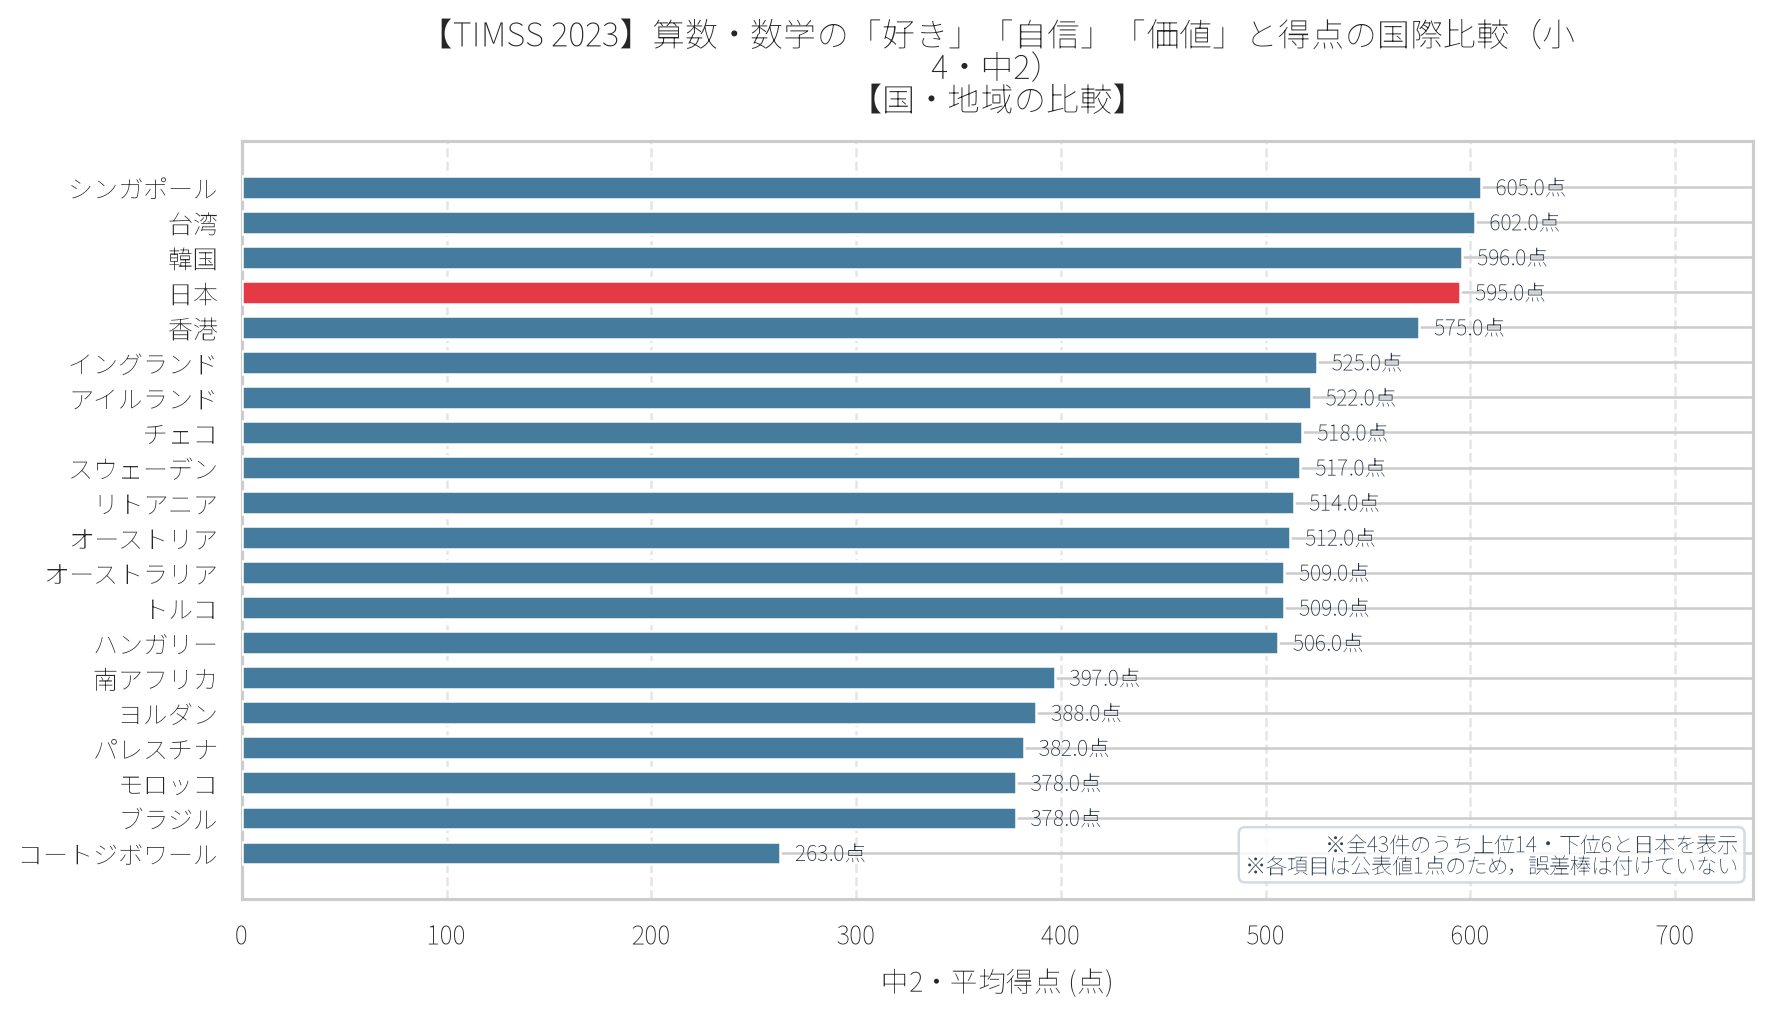
\includegraphics[width=\columnwidth]{chart_timss2023_student_attitudes.png}\caption{中2・平均得点の値の比較（上位・下位と日本を抜粋）}\end{figure}
\begin{figure}[t]\centering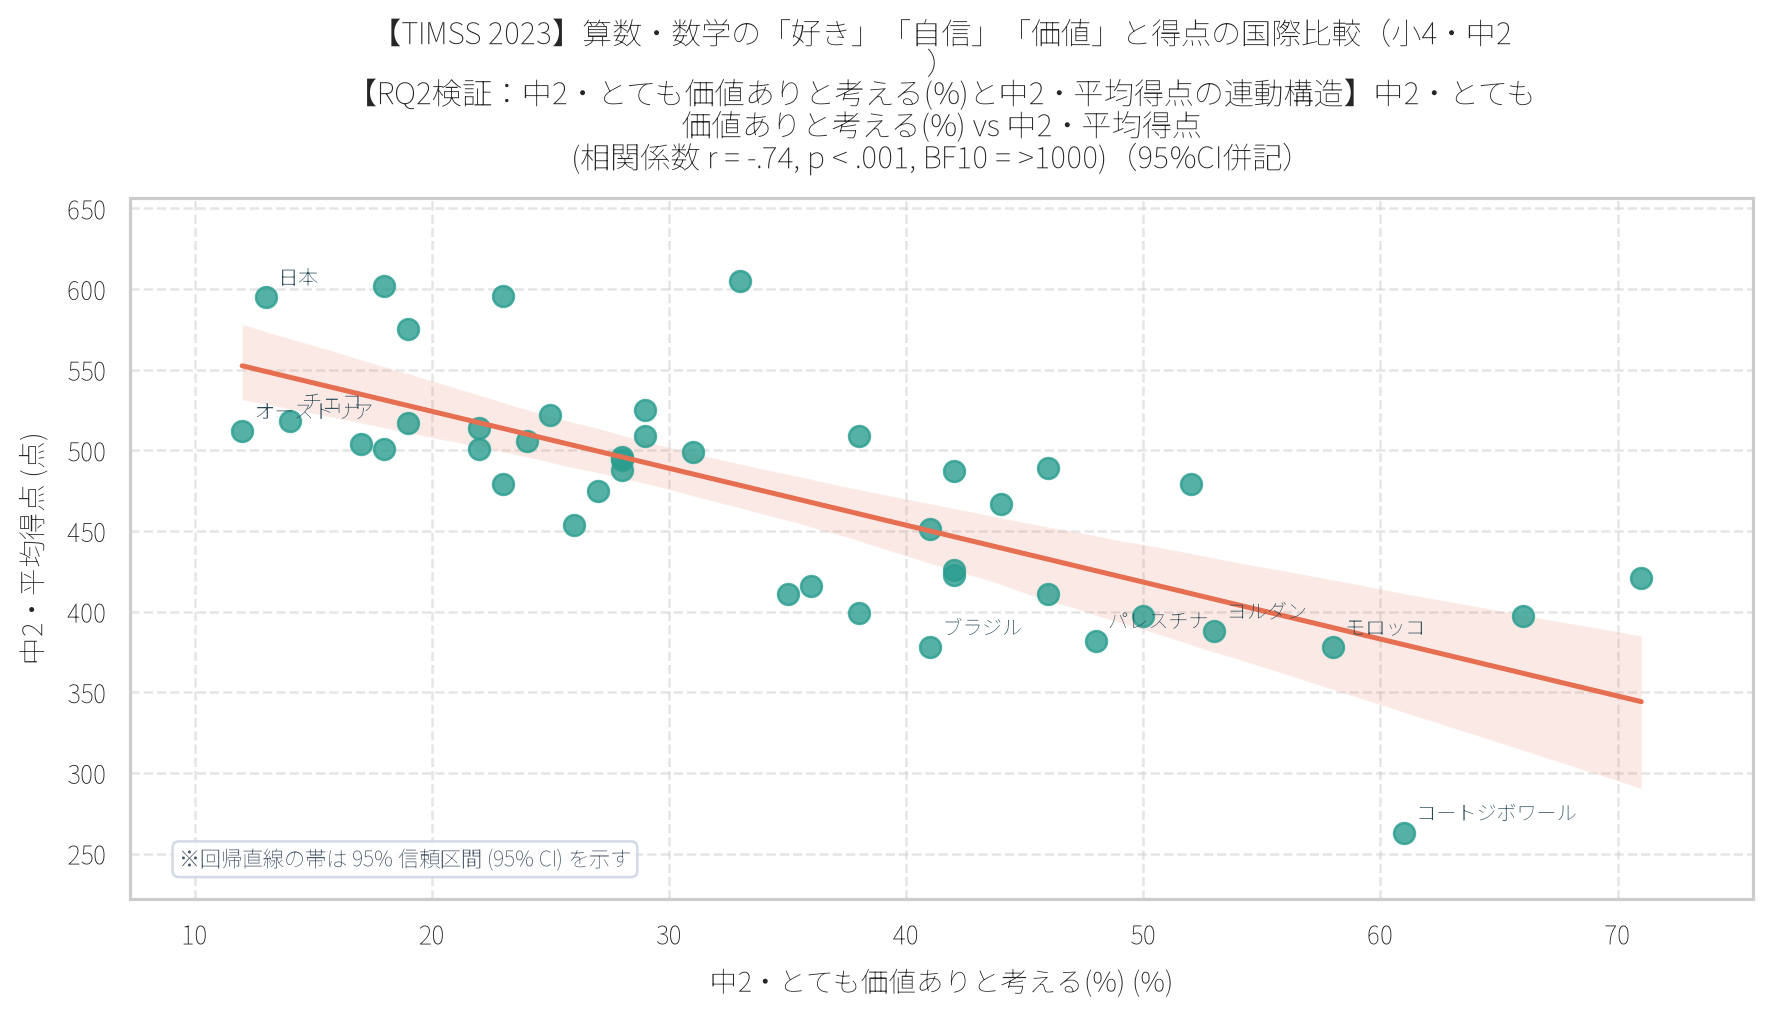
\includegraphics[width=\columnwidth]{chart_secondary_timss2023_student_attitudes.png}\caption{中2・とても価値ありと考える(\%)と中2・平均得点の関連（回帰直線と95\%信頼区間の帯）}\end{figure}
\begin{table}[t]
\caption{中2の平均得点を従属変数とした重回帰分析}
\centering\scriptsize\setlength{\tabcolsep}{3pt}
\begin{tabular}{>{\raggedright\arraybackslash}p{3.0cm}rrrr}
\toprule
説明変数 & $\beta$ & 95\%CI & \textit{p} & VIF \\
\midrule
「とても好き」の割合 & $+$0.17 & [$-$0.45, $+$0.81] & 0.533 & 7.30 \\
「とても自信あり」の割合 & $+$0.24 & [$-$0.01, $+$0.49] & 0.023 & 1.04 \\
「とても価値あり」の割合 & $-$0.93 & [$-$1.61, $-$0.35] & 0.002 & 7.41 \\
\bottomrule
\end{tabular}
\par\smallskip{\scriptsize 注）従属変数：中2・平均得点．\textit{n}=43，\textit{R}\textsuperscript{2}=0.60（調整済み 0.57），\textit{F}(3,39)=19.59．標準化係数．95\%CIはブートストラップ（2000回）．}
\end{table}
\begin{table}[t]
\caption{パス解析：直接・間接・総合の関連（標準化）}
\centering\scriptsize\setlength{\tabcolsep}{3pt}
\begin{tabular}{>{\raggedright\arraybackslash}p{3.4cm}rrr}
\toprule
経路 & 直接 & 間接 [95\%CI] & 総合 \\
\midrule
「とても好き」の割合 → 平均得点（中2） & 0.00 & -0.72 [-0.81, -0.59] & -0.72 \\
\bottomrule
\end{tabular}
\par\smallskip{\scriptsize 注）\textit{$\chi^2$}(2)=1.88，RMSEA=0.00，CFI=1.00（観測数が少ないため目安）．間接の95\%CIはブートストラップ（2000回）．「直接」が0.00の経路は，モデルに含めていない．}
\end{table}
\begin{figure*}[t]\centering
\begin{tikzpicture}[>=stealth,node distance=1cm,
  obs/.style={draw,rounded corners=2pt,minimum height=1.0cm,text width=3.8cm,align=center,font=\footnotesize},
  lat/.style={draw,ellipse,minimum height=1.0cm,text width=3.4cm,align=center,font=\footnotesize},
  lab/.style={font=\scriptsize,fill=white,inner sep=1pt}]
  \node[obs] (n1950836542) at (1.40,1.00) {「とても好き」の割合};
  \node[obs] (n2805643326) at (1.40,-1.00) {「とても自信あり」の割合};
  \node[obs] (n2430286301) at (6.27,0.00) {「とても価値あり」の割合\\{\scriptsize $R^2$=.86}};
  \node[obs] (n2632914406) at (11.13,0.00) {平均得点（中2）\\{\scriptsize $R^2$=.60}};
  \draw[->] (n1950836542) -- node[lab,pos=0.5] {.93***} (n2430286301);
  \draw[->] (n2430286301) -- node[lab,pos=0.5] {−.77***} (n2632914406);
  \draw[->] (n2805643326) -- node[lab,pos=0.5] {.24*} (n2632914406);
\end{tikzpicture}
\caption{パス図（標準化係数。破線は \textit{p}$\ge$.05。\textit{n}=43）}
\end{figure*}
\begin{figure*}[t]\centering
\begin{tikzpicture}[>=stealth,
  obs/.style={draw,rounded corners=2pt,minimum height=0.9cm,text width=1.69cm,align=center,font=\tiny,inner sep=2pt},
  lat/.style={draw,ellipse,minimum height=1.2cm,text width=2.36cm,align=center,font=\footnotesize,inner sep=1pt},
  lab/.style={font=\scriptsize,fill=white,inner sep=1pt}]
  \node[lat] (n1828638323) at (3.88,0.00) {肯定的な回答の多さ};
  \node[obs,text width=3.52cm,font=\scriptsize] (n2805643326) at (9.30,1.70) {「とても自信あり」の割合};
  \node[obs,text width=3.52cm,font=\scriptsize] (n2632914406) at (13.56,0.00) {平均得点（中2）};
  \node[obs] (n1950836542) at (0.97,-2.2) {「とても好き」};
  \draw[->] (n1828638323) -- node[lab,pos=0.62] {.97} (n1950836542);
  \node[obs] (n2430286301) at (2.91,-2.2) {「とても価値あり」};
  \draw[->] (n1828638323) -- node[lab,pos=0.62] {.96} (n2430286301);
  \node[obs] (n244879145) at (4.84,-2.2) {「好きでない」};
  \draw[->] (n1828638323) -- node[lab,pos=0.62] {-.96} (n244879145);
  \node[obs] (n102540247) at (6.78,-2.2) {「価値を感じない」};
  \draw[->] (n1828638323) -- node[lab,pos=0.62] {-.89} (n102540247);
  \draw[->] (n1828638323) -- node[lab,pos=0.5] {−.73***} (n2632914406);
  \draw[->,dashed] (n2805643326) -- node[lab,pos=0.5] {.16} (n2632914406);
\end{tikzpicture}
\caption{潜在変数を含むSEM（1因子）（標準化推定値。\textit{$\chi^2$}(8)=62.87，CFI=0.83，RMSEA=0.40，\textit{n}=43。破線は \textit{p}$\ge$.05）}
\end{figure*}
\section{考察}
RQ1の結果，「好き」「価値」の割合が高い国・地域ほど平均得点が低い傾向があり，3つを同時に入れても「価値」の負の係数は残った．しかし「好き」とは \textit{r}=.93 と強く相関し，2つを分けて推定できない．上位5を除くと2つのβは小さくなったが合計は変わらず，単独の \textit{r} も不変なので，上位国への依存というより共線性による係数の配分の変化かもしれない．両者は区別できない．「自信」の関連は不安定であった．

この向きは，個人の水準で動機づけとの結びつきを想定する枠組み（Bandura (1997)，Wigfield and Eccles (2000)，Pekrun (2006)）とは逆だが，国内の差は正であり，個人の関連を否定しない．個人への当てはめは生態学的誤謬（Robinson (1950)）にあたる．考えられる理由は，Shen and Tam (2008)が示した逆説的な関係と同じ向きであること，自己評価が比べる集団に左右されるなら得点の高い国・地域で「とても」と答える割合が低くなりうること（Marsh and Hau (2003)は国内の学校間の比較で，類推にとどまる），Chen et al. (1995)が論じた回答の仕方の違いが東アジアの上位の国・地域に表れていることである．いずれも仮説で，本研究のデータでは検証できない．

パス解析の間接的な関連は，「好き→価値→得点」の順序に根拠がなく，「価値→好き→得点」など同値なモデルでも同じ適合になりうる．直接パスを置かない仮定も検定しておらず，適合の良さは因果や順序の証拠ではない．SEMの不適合は，同じ質問の別区分（合計が約100\%）の「好き」と「好きでない」，「価値」と「価値を感じない」を誤差の相関なしで入れた設定が主因とみられ，実質的な知見ではない．

「好き」や「価値」を高める取り組みの効果は確かめられていない．限界は，(1)集計値のみで個人の因果を特定できないこと，(2)自己申告で回答の仕方の違いを受けうること，(3)標本の大きさや標準誤差を扱っていないこと，(4)経済水準などの交絡を統制していないこと，(5)2023年の1時点で，Mullis et al. (2020)の2019年との変化を検討していないこと，(6)136組の探索と3つのモデルによる多重比較，(7)観測数43に説明変数3つで係数が不安定なこと，(8)国・地域が独立でなく，クックの距離がコートジボワール0.42，日本0.28と基準（0.093）を超えること，である．
\section*{参考文献}
\begingroup\scriptsize\setlength{\parindent}{0pt}\raggedright
\par\hangindent=1.5\zw\hangafter=1 BANDURA, A. (1997) Self-efficacy: The exercise of control. W. H. Freeman and Company.\vspace{1pt}
\par\hangindent=1.5\zw\hangafter=1 CHEN, C., LEE, S. and STEVENSON, H. W. (1995) Response style and cross-cultural comparisons of rating scales among East Asian and North American students. Psychological Science, \textbf{6} (3) ：170-175.\vspace{1pt}
\par\hangindent=1.5\zw\hangafter=1 IEA (2024) TIMSS 2023 International Results in Mathematics and Science. Boston College, TIMSS \& PIRLS International Study Center.\vspace{1pt}
\par\hangindent=1.5\zw\hangafter=1 LEE, J. and STANKOV, L. (2018) Non-cognitive predictors of academic achievement: Evidence from TIMSS and PISA. Learning and Individual Differences, \textbf{65} ：50-64.\vspace{1pt}
\par\hangindent=1.5\zw\hangafter=1 MARSH, H. W. and HAU, K.-T. (2003) Big-fish--little-pond effect on academic self-concept: A cross-cultural (26-country) test of the negative effects of academically selective schools. American Psychologist, \textbf{58} (5) ：364-376.\vspace{1pt}
\par\hangindent=1.5\zw\hangafter=1 MULLIS, I. V. S., MARTIN, M. O., FOY, P., KELLY, D. L. and FISHBEIN, B. (2020) TIMSS 2019 International Results in Mathematics and Science. Boston College, TIMSS \& PIRLS International Study Center.\vspace{1pt}
\par\hangindent=1.5\zw\hangafter=1 PEKRUN, R. (2006) The control-value theory of achievement emotions: Assumptions, corollaries, and implications for educational research and practice. Educational Psychology Review, \textbf{18} (4) ：315-341.\vspace{1pt}
\par\hangindent=1.5\zw\hangafter=1 ROBINSON, W. S. (1950) Ecological correlations and the behavior of individuals. American Sociological Review, \textbf{15} (3) ：351-357.\vspace{1pt}
\par\hangindent=1.5\zw\hangafter=1 SHEN, C. and TAM, H. P. (2008) The paradoxical relationship between student achievement and self-perception: a cross-national analysis based on three waves of TIMSS data. Educational Research and Evaluation, \textbf{14} (1) ：87-100.\vspace{1pt}
\par\hangindent=1.5\zw\hangafter=1 WIGFIELD, A. and ECCLES, J. S. (2000) Expectancy-value theory of achievement motivation. Contemporary Educational Psychology, \textbf{25} (1) ：68-81.\vspace{1pt}
\endgroup
\section*{Summary}
{\footnotesize\setlength{\parindent}{0pt}Using published TIMSS 2023 values for 43 countries and economies, we examined how the shares of Grade 8 students who very much like, are very confident in, and highly value mathematics relate to average mathematics scores. Japan ranked 4th in score (595). Taken one at a time, liking (r = -.67) and value (r = -.74) were negatively correlated with scores, while no association was found for confidence (r = .12). In a multiple regression with all three, the standardized coefficient for value was -.933 (95\% CI [-1.61, -.35]) and that for liking was .172 (95\% CI [-.45, .81]); the two shares were strongly correlated (r = .93, VIF about 7.4), so their separate roles could not be distinguished. The path model fitted well (CFI = 1.000), but the SEM, which combined complementary response categories without error correlations, fitted poorly (CFI = .832, RMSEA = .399). All results are associations between country-level aggregates and do not show causation for individual students.\par\smallskip KEYWORDS: TIMSS 2023, Learning Motivation, Multiple Regression, Path Analysis, Structural Equation Modeling\par}
\medskip\noindent\fbox{\parbox{\dimexpr\columnwidth-2\fboxsep-2\fboxrule}{\footnotesize\gtfamily 【付記：生成AIによる自動執筆に関する開示】\\ 本論文は学生への教育目的で作成している．使用しているデータは公的オープンデータである．統計の算出はPythonで行い，文章は生成AI（Anthropic Claude等）を活用して作成した．記載した統計数値は元データに準拠しているが，教育学的な考察や提言の妥当性は，指導現場の実情に応じて，批判的に吟味してほしい．}}
\end{document}
